% !TeX spellcheck = de_DE
{\setbeamertemplate{frame footer}{\textit{Bildquelle:} NASA}
\begin{frame}{Motivation}
	\begin{columns}[c,onlytextwidth]
		\column{0.6\textwidth}
		\alert{Problem}
		\begin{itemize}
			\item Raumsonde zum Pluto:\\
			Wartezeit auf Fotos verkürzen\pause
			\item Alltäglicher:\\
			Hochaufgelöste Fotos per Mail
		\end{itemize}\pause[1]
		
		\column{0.4\textwidth}
		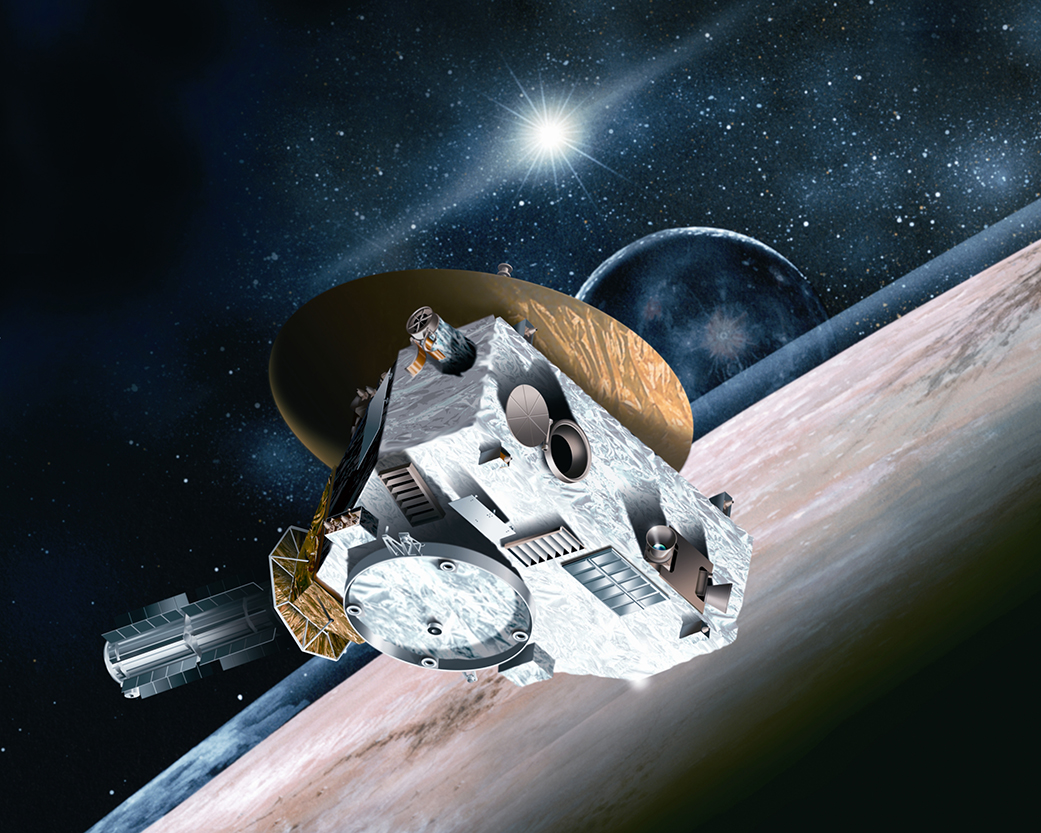
\includegraphics[width=\textwidth]{newHorizons.jpg}
	\end{columns}\vspace{-1mm}\pause[3]
	\alert{Lösung}\vspace{-2mm}
	\begin{description}
		\item [verlustfreie Kompression:]  \hspace{48mm}$\rightarrow$ PNG\\
		\hspace{-14.4mm}Maximiere Entropie\ \ \ $\Rightarrow$\ \ \ $\exists$ untere Schranke\pause
		\item [verlustbehaftete Kompression:] \hspace{39mm}$\rightarrow$ JPEG\\
		\hspace{-14.4mm}Unterteile Informationen in Detailstufen\\
		\hspace{-20.2mm}$\Rightarrow$\hspace{1.1mm} beste Auflösung bei gegebenem Speicherplatz
	\end{description}
\end{frame}}

\begin{frame}{Gliederung}
	\setbeamertemplate{section in toc}[sections numbered]
	\tableofcontents[hideallsubsections]
\end{frame}

\section[Multiskalenanalyse \hspace{42mm}\small am Beispiel der eindimensionalen Haar-Wavelets]{Multiskalenanalyse}
	
	\begin{frame}{Mathematisches Modell: Die Multiskalenanalyse}
		\alert{Konstruktion}
		\begin{enumerate}
			\item geschachtelte Vektorräume:\hspace{16.5mm}$V_0\subset V_1\subset ...\subset V_N$\vspace{2mm}
			\item[$\Leftrightarrow$\hspace{-0.3mm}] {\bf Skalenfunktionen} (Basen der $V_i$):\hspace{8mm}$\{\phi^i_1, ..., \phi^i_{\dim V_i}\}=:\Phi^i$\vspace{2mm}\pause
			\item Skalarprodukt auf $V_N$:\hspace{27.2mm}$\|\cdot\|_{ind}\ \widehat{=}$ Fehlermaß\vspace{2mm}
			\item[$\Rightarrow$\hspace{-0.3mm}] orthogonale Komplemente $W_i$:\hspace{12mm}$W_i\oplus V_i=V_{i+1}$\vspace{2mm}\pause
			\item {\bf Wavelets} (Basen der $W_i$):\hspace{21.5mm}$\{\psi^i_1, ..., \psi^i_{\dim W_i}\}=:\Psi^i$
		\end{enumerate}
	\end{frame}

	\begin{frame}{Wavelet-Transformation I}
		\alert{Basiswechsel} von $V_{i}$ nach $V_{i-1}\oplus W_{i-1}$: \vspace{2mm}\[ \left[ \Phi^i\right] =\left[ \Phi^{i-1}\mid \Psi^{i-1}\right]\left[ \frac{\ A^i\ }{\ B^i\ }\right];\qquad T^i_{sf\rightarrow wl}=:\left[ \frac{\ A^i\ }{\ B^i\ }\right]\pause[2]=:\left[ P^i\mid Q^i\right]^{-1}\vspace{3mm}\]\pause[3]
		$\Rightarrow\qquad \begin{cases}
			&A^i\cdot C^i=C^{i-1}\vspace{2mm}\\
			&B^i\cdot C^i=D^{i-1}
		\end{cases}$\vspace{10mm}\\
		$C^i$: Koeffizientenvektor in $V_i$\hspace{8.8mm} $D^i$: Detailkoeffizienten in $W_i$\vspace{2mm}\\ \pause[1]
		$A^i$, $B^i$: {\bf Analyse Filter}\hspace{22mm}\pause[2] $P^i$, $Q^i$: {\bf Synthese Filter}
	\end{frame}

	\begin{frame}{Wavelet-Transformation II}
		\alert{\bf Filter Bank:}\\rekursive Ausführung der Analyse Filter\vspace{10mm}\\
		{\centering\includegraphics[page=11, trim=60 695 305 100, clip, width=0.9\textwidth]{4_wavelet_final[14255].pdf}\vspace{12mm}}\\ \pause
		\large$\Rightarrow$\qquad Darstellung von\ \ $V_N$\ \ als\ \ $\bigoplus_{i=0}^{N-1}W_i\oplus V_0$
	\end{frame}

	{\setbeamertemplate{frame footer}{\textit{Bildquelle:} wikipedia.org}
	\begin{frame}{Wahl der Skalenfunktionen und Wavelets}
		\begin{columns}[T, onlytextwidth]
			\column{0.25\textwidth}
			\alert{Ziel}\vspace{3.2mm}\\
			\ \ \ \ \ \ \ Wavelets ...
			\column{0.6\textwidth}
			\begin{itemize}
				\item[...] mit kleinem Träger,\item[...] orthonormal,\item[...] k-mal stetig differenzierbar
			\end{itemize}
		\end{columns}\pause
		\begin{columns}[c, onlytextwidth]
			\column{0.55\textwidth}\vspace{-6mm}
			\begin{description}
				\item[\alert{\sf Bestmöglich umgesetzt}] \ \\ \hspace{-14.4mm}Daubechies-Wavelets\vspace{3mm}\pause
				\item[\alert{\sf JPEG-2000-Format}] \ \\ \hspace{-14.4mm}Cohen–Daubechies–Feauveau\\ \hspace{-14.4mm}5/3 und 9/7 Wavelets
			\end{description}\pause
			\column{0.4\textwidth}\vspace{2mm}
			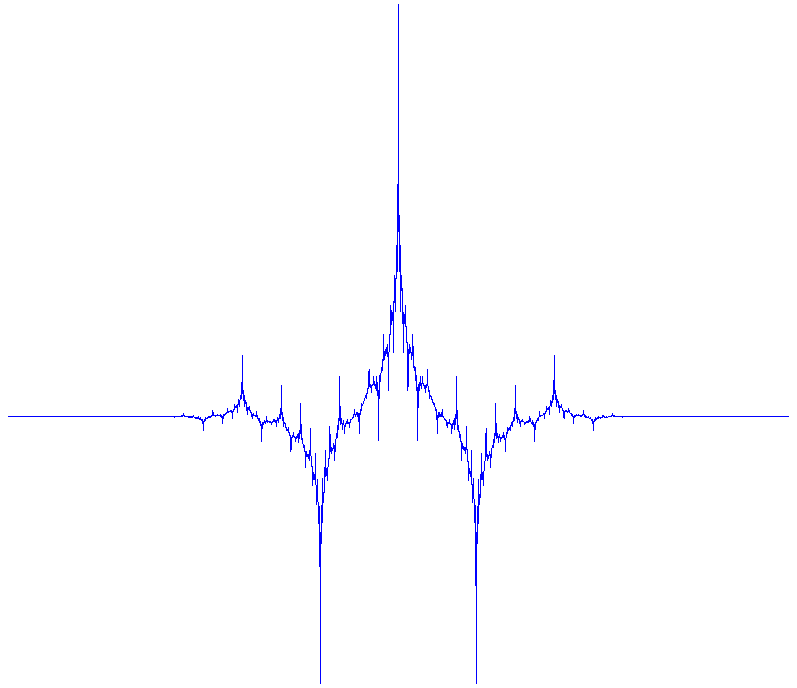
\includegraphics[width=\textwidth]{CDFWavelet.pdf}
		\end{columns}
	\end{frame}}


\section{Wavelet-Kompression}

	\begin{frame}{2D Wavelets}
		\begin{columns}[T,onlytextwidth]
			\column{0.4\textwidth}
			{\bf Vektorräume}\vspace{3mm}\\
			{\bf Skalarprodukt}\vspace{3mm}\\
			{\bf Skalenfunktionen}
			\column{0.6\textwidth}\vspace{-1mm}
			$V^i_{2D}:= V^i_{1D}\times V^i_{1D}\subset\left[ \mathcal{L}^2([0,1])\right]^2$\vspace{3mm}\\
			$\left\langle f, g\right\rangle _{2D}:=\int_{0}^{1}\int_{0}^{1}f(x,y)g(x,y)\mathsf{d}x\mathsf{d}y$\vspace{3mm}\\
			$\Phi^i_{2D}(x, y):=\{\phi^i_k(x)\phi^i_l(y)\mid \phi^i_k, \phi^i_l\in\Phi^i_{1D} \}$
		\end{columns}\vspace{4mm}\pause
		\begin{center}
				\bf Wavelets\vspace{-4mm}
		\end{center}
		\alert{Standard-Konstruktion}\vspace{1mm}\\
		\hspace{12mm}$\Psi^i_{2D}(x, y):=\{\psi^i_k(x)\psi^i_l(y)\mid \psi^i_k,\psi^i_l\in\Phi_{1D}^0\cup\Psi_{1D}^0\cup...\cup\Psi_{1D}^{i} \}$\vspace{3mm}\\ \pause
		\alert{Nicht-Standard-Konstruktion}\vspace{1mm}\\
		\hspace{12mm}$\tilde\Psi^i_{2D}(x, y):=\{2^i\psi^0(2^ix-k, 2^iy-l)\mid \psi^0 \in \Psi^0_{2D}\}$
	\end{frame}

	{\setbeamertemplate{frame footer}{\textit{Bildquelle:} Wavelets for Computer Graphics: A Primer}
	\begin{frame}{2D Haar-Wavelets}
		\begin{columns}[T, onlytextwidth]
			\column{0.46\textwidth}
			\centering
			\alert{Standard-Wavelets}\vspace{4mm}\\
			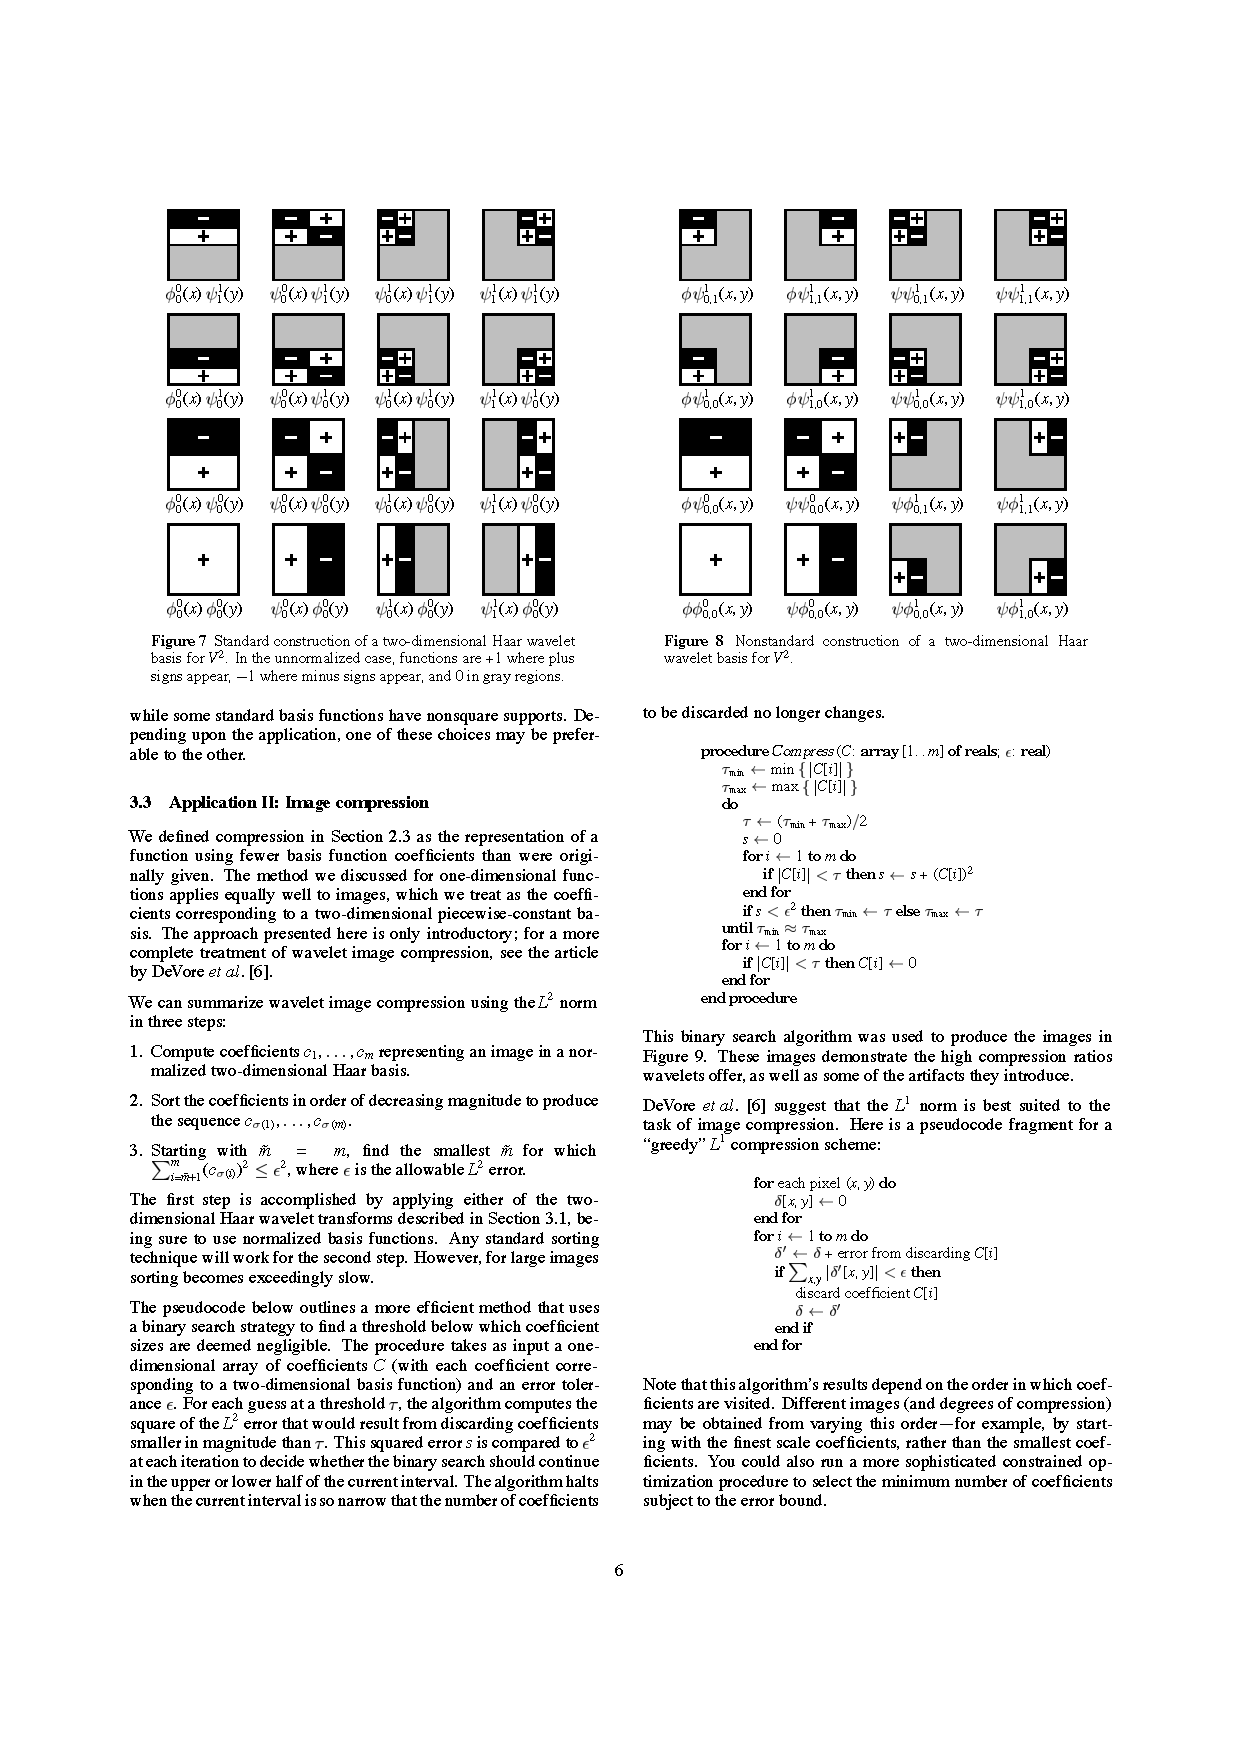
\includegraphics[trim=79 545 325 100, clip, width=\textwidth]{2d_wavelets.pdf}
			\column{0.46\textwidth}
			\centering
			\pause
			\alert{Nicht-Standard-Wavelets}\vspace{4mm}\\
			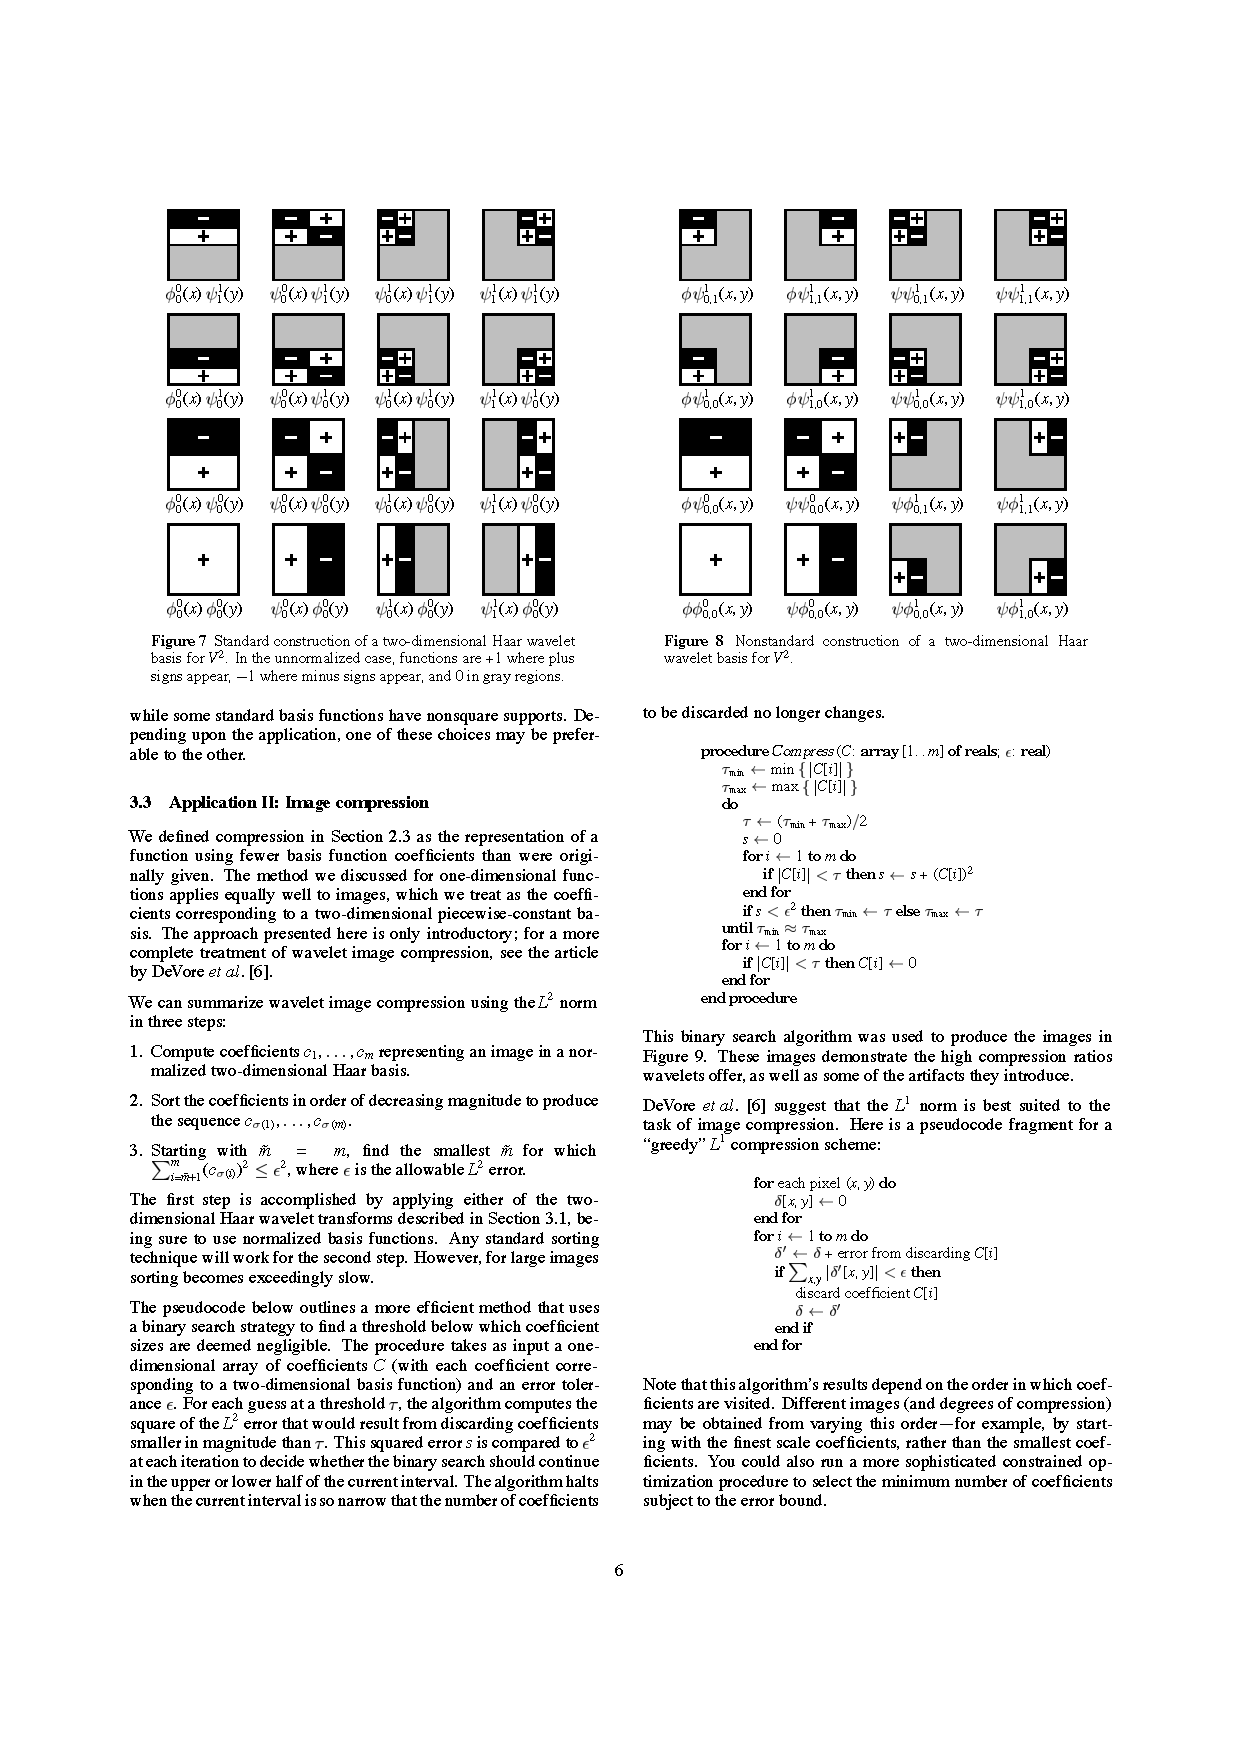
\includegraphics[trim=325 545 79 100, clip, width=\textwidth]{2d_wavelets.pdf}
		\end{columns}
	\end{frame}}

	{\setbeamertemplate{frame footer}{\textit{Bildquelle:} NASA}
	\begin{frame}{Kompression: Skalenfunktionen vs. Wavelets}
		\begin{columns}[T, onlytextwidth]
			\column{0.46\textwidth}
			\centering
			\alert{Skalenfunktionen}\vspace{4mm}\\
			\includegraphics<1>[width=\textwidth]{zPluto1.png}
			\includegraphics<2>[width=\textwidth]{zPluto2.png}
			\includegraphics<3>[width=\textwidth]{zPluto4.png}
			\includegraphics<4>[width=\textwidth]{zPluto8.png}
			\includegraphics<5>[width=\textwidth]{zPluto16.png}
			\includegraphics<6>[width=\textwidth]{zPluto32.png}
			\includegraphics<7>[width=\textwidth]{zPluto64.png}
			\includegraphics<8>[width=\textwidth]{zPluto128.png}
			\includegraphics<9>[width=\textwidth]{zPluto256.png}
			\includegraphics<10>[width=\textwidth]{zPluto512.png}
			\includegraphics<11>[width=\textwidth]{Pluto1k.png}
			\column{0.46\textwidth}
			\centering
			\alert{Wavelets}\vspace{4mm}\\
			\includegraphics<1>[width=\textwidth]{Pluto1.png}
			\includegraphics<2>[width=\textwidth]{Pluto2.png}
			\includegraphics<3>[width=\textwidth]{Pluto4.png}
			\includegraphics<4>[width=\textwidth]{Pluto8.png}
			\includegraphics<5>[width=\textwidth]{Pluto16.png}
			\includegraphics<6>[width=\textwidth]{Pluto32.png}
			\includegraphics<7>[width=\textwidth]{Pluto64.png}
			\includegraphics<8>[width=\textwidth]{Pluto128.png}
			\includegraphics<9>[width=\textwidth]{Pluto256.png}
			\includegraphics<10>[width=\textwidth]{Pluto512.png}
			\includegraphics<11>[width=\textwidth]{Pluto1k.png}
		\end{columns}
	\end{frame}}

	\begin{frame}{Verlustbehaftete Kompression}
		\begin{description}[r]
			\item[\alert{\sf Gegeben\ }]$f=\sum_{i=1}^{n}c_iu_i\in V_N$\ \ mit ONB\ \ $\{u_i\mid 1\leq i\leq n\}$\vspace{3mm}\pause
			\item[\alert{\sf Gesucht\ \ }]Näherung \ $\tilde{f}$ \ von \ $f$\ \ mit \ $m<n$ \ Koeffizienten\\ \hspace{16mm}$\Rightarrow$\ \ $c_i=0\quad\forall m+1\leq i\leq n$
		\end{description}\vspace{-2mm}\pause
		\begin{align*}
		||f-\tilde{f}||_2^2	= \left\langle \sum_{i =m+1}^n c_i u_i , \sum_{j =m+1}^n c_j u_j \right\rangle
		= \sum_{i,j =m+1}^n c_i c_j \left\langle  u_i , u_j \right\rangle 
		= \sum_{i =m+1}^n c_i^2
		\end{align*}\ \vspace{1.5mm} \\ \pause
		\alert{Bestmögliche Kompression}\vspace{1mm}\\ \hspace{18mm}1.\quad Sortiere die $c_i$ von groß nach klein\\ \hspace{18mm}2.\quad Verwende nur die ersten $m$ Koeffizienten
	\end{frame}

